\documentclass{sig-alternate-05-2015}
\usepackage[colorlinks=true,linkcolor=black]{hyperref}
\begin{document}
\numberofauthors{5}
\title{Computer Science 145 Final Project Report}
\date{March 20th, 2019}
\author{
    \alignauthor
    Alexander Chen\\
    \affaddr{UID: 404837697}\\
    \email{aqchen@g.ucla.edu}\\
    \alignauthor
    Danny Nguyen\\
    \affaddr{UID: 004628653}\\
    \email{dannydatnguyen@ucla.edu}\\
    \and
    \alignauthor
    Michael Wu\\
    \affaddr{UID: 4047517542}\\
    \email{michaelwu756@gmail.com}\\
    \alignauthor
    Jennie Zheng\\
    \affaddr{UID: 304806663}\\
    \email{yzheng7@g.ucla.edu}\\
    \alignauthor
    Yijing Zhou\\
    \affaddr{UID: 404786683}\\
    \email{yijingz1227@gmail.com}\\
}
\maketitle

\begin{abstract}
In this project we attempt to predict what a user would rate a movie based on the user's past
movie ratings. We tested various machine learning models and data processing methods in order to
perform this task. Our data consisted of a set of movie ratings for each user and information
about a movie's genome. We analyzed this data using neural networks, random forest, SVD ensembles,
and gradient boosted trees. Our predictions were submitted to a class-wide Kaggle competition
that would score our submissions. We ranked 10th. Our most successful model was our 50 instance
SVD ensemble which produced a RMSE of 0.841 on the testing data.
\end{abstract}

\section{Introduction}

Movie recommendations are vital for customers to quickly find the movies they'd like to watch. Companies
like IMDb, Netflix, and MovieLens all include a recommendation system where users can find potential
movies given their previous browsing history and ratings. These companies are able to build user
profiles and further improve their recommendation system with this information. These recommendation
systems have a large business impact since they keep users on company's website and improve overall
customer satisfaction. The recommendation system on YouTube keeps users on the website
which directly translates to increased ads views and revenue. For Netflix, the recommendation system
improves the user experience and simplifies content discovery. In this project, we create a movie rating prediction
model. This model predicts the rating a given user would give to a particular movie. This type of model is the basis
for many recommendation systems that have become integral to modern video and movie platforms.

\section{Related Work}

The work described in this report is part of a larger body of work on recommendation systems, which include Yelp
restaurant tips, Tinder partner suggestions, and Youtube video recommendations.

Common approaches to recommendation systems include collaborative filtering, content-based filtering,
as well as hybrid methods. Collaborative filtering emphasises the users, and predicts how much
a particular user will like a product based on the user's similarity in preferences and behaviors to
other users. It's based on the idea that users who agree often will continue to agree. Content-based
filtering focuses on the product. It makes predictions using a user's behaviors and preferences
towards other products. Hybrid systems unify these two approaches, and the methods in this report mainly
use a hybrid approach.

Our problem is very similar to that of the Netflix Prize, a famous large-scale data science competition
hosted by Netflix to improve their recommendation system. The winner receives \$1,000,000,
which shows how important recommendation system are in online movie platforms.

\section{Problem Definition and Formulation}

In this project, we are given a data set consisting of several CSV files that include movie metadata,
user ratings, and movie genome tags. This data set is split into labeled training data and unlabeled
testing data. Using all of this information, we want to evaluate several different
models so that we can answer the following question: given an unseen test \{user, movie\} pair, what would the
user rate that particular movie? Our predictions were compared against the true ratings
of the test data on Kaggle using RMSE.

We approach this problem by reading the necessary data from the provided CSV files, visualizing this data for
insight, then processing the data into a feature vectors. Next, we iteratively
train and tune multiple models using our training data and use each model to predict ratings for the validation
and test data. We evaluate these predictions using RMSE to choose the best model.

\section{Data Preparation}

\subsection{Visualization}

\begin{figure}
    \begin{center}
        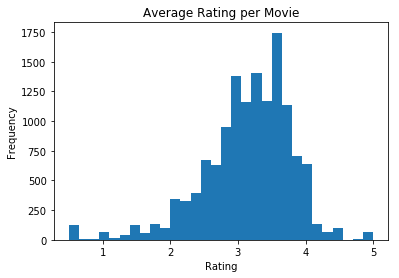
\includegraphics[width=2in]{AverageRatingByMovie.png}
        \caption{The average rating per movie is centered between three and four.}
        \label{averagemovieratings}
    \end{center}
\end{figure}

The average rating across all \{user, movie\} pairs in the training data is about 3.535 as depicted in
figure \ref{averagemovieratings}. This is interesting to note because the average rating is higher than 3, which
is the middle of the range \([1,5]\). This could be due to selection bias or other factors.
Because of this, we decided to normalize our data around the mean during the data processing stage.

\begin{figure}
    \begin{center}
        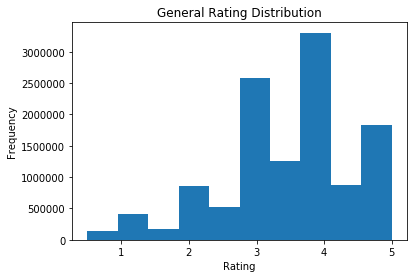
\includegraphics[width=2in]{RatingHistogram.png}
        \caption{Users tend to give full rather than half scores, and the ratings have negative skew.}
        \label{ratingdistribution}
    \end{center}
\end{figure}

Since users can only give ratings in increments of 0.5 as shown in figure \ref{ratingdistribution}, we discussed
whether we should round our predictions. Then we could approach this task as either a classification problem or
a regression problem. For classification, we would produce values in the following set.
\[\{0.5,1,1.5,2,2.5,3,3.5,4,4.5,5\}\]
This seemed reasonable because users could only give these exact scores, but since we aimed to minimize RMSE we
decided to approach this task as a regression problem and not round our predictions. RMSE punishes larger errors
more than smaller ones, so classification algorithms would not be a good fit since they assume that any error
has the same loss. We later tested this hypothesis and found that providing real values rather than rounded ones
results in lower RMSE.

\begin{figure}
    \begin{center}
        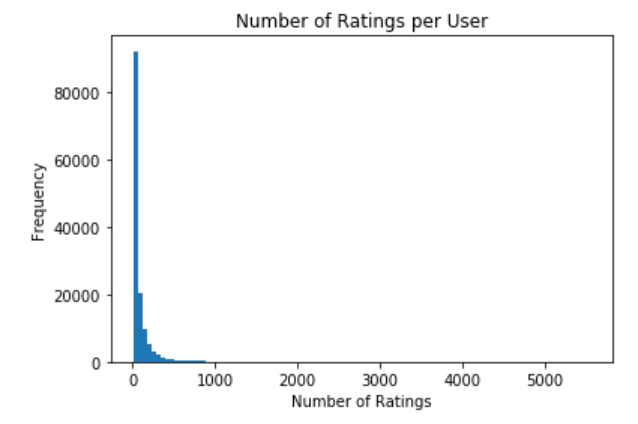
\includegraphics[width=2in]{NumRatingsPerUser.png}
        \caption{Since a few individuals rate a large number of movies, the data is skewed right. The median
        number of ratings per user is 40 and the mode is 12.}
        \label{ratingsperuser}
    \end{center}
\end{figure}

Since the typical user does not rate that many movies, as shown in figure \ref{ratingsperuser}, an approach that separates
data based on each user may not be sufficient. This is because a particular user may simply not have enough data
to make accurate predictions.

\begin{figure}
    \begin{center}
        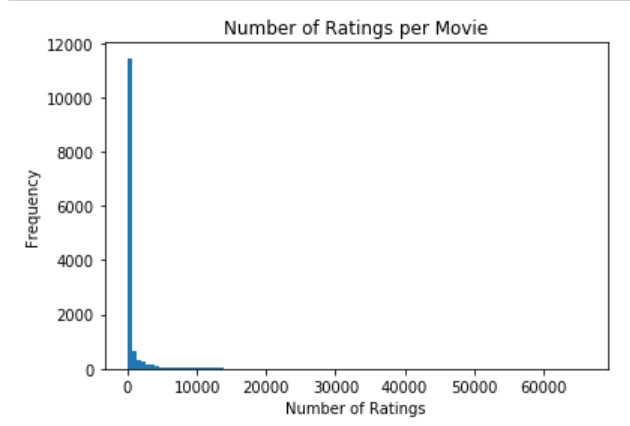
\includegraphics[width=2in]{NumRatingsPerMovie.png}
        \caption{Since a few movies receive a large number of ratings, the data is skewed right. The median number of
        ratings per movie is 27 and the mode is 1.}
        \label{ratingspermovie}
    \end{center}
\end{figure}

Since the typical movie also does not receive many ratings, an approach that separates
data based on each movie may also not be sufficient. As a result, a hybrid approach that learns from all the given
information about the movies and the users is necessary for our prediction model.

\subsection{Feature Vector Generation}

First we generated feature vectors for each movie and each user using the movie genomes and the movie ratings for each user. The
feature vector for each movie was its genome score. There were 1128 genome tags, so the feature vector was 1128 values long. The user
feature vector consisted of the weighted average of the feature vectors of all the movies that the user rated. We weighted
each movie by multiplying its feature vector with the user rating normalized around the mean. Any missing values were set to zero.

For each movie and user pair, we generated a feature vector which the element-wise multiplication between the user vector and movie vector.
We used these feature vectors as the training data for our models.

We faced major performance issues when processing our data and training our models since the training data had 11 million examples.
Due to the size of the data, when we attempted to create feature vectors for each example we had to utilize lazy loading and
accessing to avoid running out of memory. Even after we began using these methods, we often faced memory errors during training.
This struggle was mitigated when we implemented Spark to handle our large data set. We also began running our code on Amazon EC2 instances
that had up to 768 Gb of memory.

Furthermore, we also tried to use the word2vec model to generate feature vectors of size 300.
With this approach we start by working with the movie genome tag vectors. Each of the 1128 tags is associated with some word or phrase.
We will convert each word or phrase to a size 300 vector, and then we can represent each movie as the weighted sum of those word vectors.
For example, let a movie have the following tags.
\begin{verbatim}
{"007": 0.8, "Action": 0.9,..., "Boring": 0}
\end{verbatim}
Then the movie feature vector can be calculated by multiplying the tag value by the word vector for that tag and averaging across
all tags. Then our feature vector will be a vector space of size 300, which leads to a \(\frac{2}{3}\) reduction in dimension.
Similarly, the user vector would be calculated by taking the weighted average movie vector in the same manner as before
and the reduction in dimension is also applied.

Since there was not sufficient time nor enough text to train the word2vec model in the time frame of this project,
we used a pre-trained word2vec model. This was based on text from Google News, which contained 3 million 300-dimension word vectors
for English words. Each tag is transformed into a 300-dimension word vector using the following principles.
\begin{enumerate}
    \item If a tag can be found in the vocabulary in the model, we use the found word vector.
    \item For tags that are phrases, we ignore certain words such as ``and'' and ``of'' and sum the word vectors from the remaining words.
    \item If we cannot generate a word vector using the previous methods, we use the zero vector.
\end{enumerate}
Then we generated the training and test feature vectors by using element-wise multiplication of the user vector and movie vector as previously
described.

Lastly, we attempted to run principle component analysis on our feature vectors for each user and movie pair. This allowed
us to reduce the size of our feature vector. We were only able to briefly use principle component analysis and did not generate
any significant results with it since we ran out of time.

\section{Learning Methods}

We designed and trained multiple different models on our processed data for our movie rating prediction task. These models are described below.

\subsection{Averaging}

Our first attempt at predictions was taking the average rating that a user gives and the average rating that a movie receives and predicting
the average of these two values. We obtained a RMSE of around 0.93 using this method on the test data.

\subsection{Linear Regression}

Our next approach was to utilized sklearn to train a simple linear regression model on our size 1128
feature vector. This resulted in a highest accuracy of 0.93. We tuned some regularization coefficients
but was ultimately unable to achieve anything better than this, since linear regression is a fairly simple
model.

\subsection{Random Forest}

We first trained a random forest of decision trees on a 1\% sample of our size 1128 feature vector data
in order to evaluate its performance. We set the number of trees to be 10 and the max depth of the trees was 5.
We were able to achieve a RMSE of 0.91 using this method, which was better than our averaging score. Afterwards
we decided to train on a larger sample of our data with 40 trees and max depth 20, which gave us a RMSE
of around 0.89.

\subsection{Gradient Boosted Trees}

Since we already wrote code in sklearn to train a random forest regressor, we were able to easily
change our classifier to use gradient boosted trees. With this method we were able to achieve a RMSE
of around 0.91. This was worse than our random forest regressor so we decided to move on.

\subsection{Word2Vec}

For the data generated by word2vec approach, we made predictions using multi-layer neural networks and \(k\)-nearest neighbours (\(k\)-NN).
Since these two models can take a long time to train (neural net) or predict (\(k\)-NN), we trained them on a 10\% sample of the training
data set to observe their performance.

For neural network, the activation functions we tested were ReLU, leak ReLU, and log softmax. We used RMSE as the loss function since
this was the one used in the Kaggle competition. We varied the architecture of the network, but the results were systematically poor
under different architectures. The first architecture we have tried had two fully connected hidden layers, each of size 32. Both
layers used ReLU as their activation functions.
\begin{figure}
    \begin{center}
        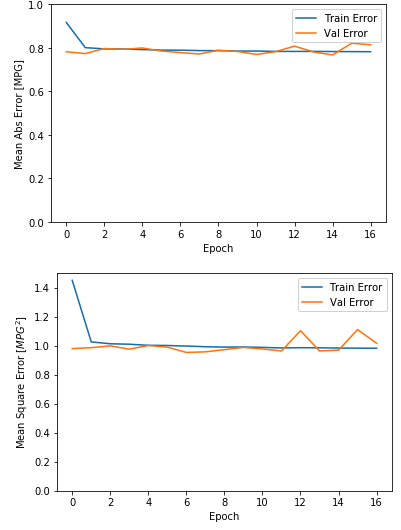
\includegraphics[width=2in]{NN32.png}
        \caption{Mean squared error and mean absolute error for neural with two hidden layers of size 32.}
        \label{neuralnet32}
    \end{center}
\end{figure}
As shown in figure \ref{neuralnet32}, the neural network is unable to further improve loss function after 16 epochs.
The improvements are negligible after 6 epochs.

The second architecture had the same layer shape as first architecture, except both layers used the log softmax activation function.
\begin{figure}
    \begin{center}
        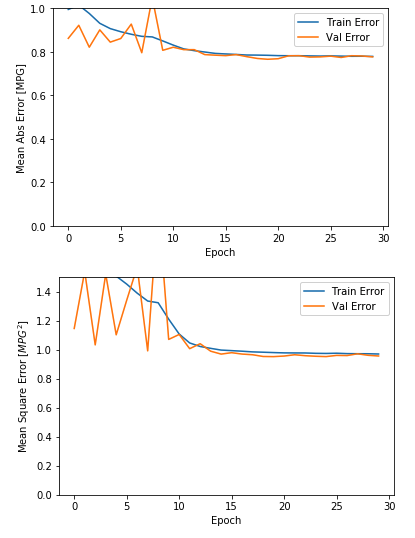
\includegraphics[width=2in]{NNSoftmax.png}
        \caption{Mean squared error and mean absolute error for Neural Net with log softmax.}
        \label{neuralnetlog}
    \end{center}
\end{figure}
This architecture took more epochs to converge and terminated at around 0.97 RMSE.
The last architecture we have tried involved four hidden layers with sizes 301, 101, 65, and 37. Again, the resulting
RMSE from the neural net prediction was poor. It is also difficult to interpret what we learn from the neural net.

\begin{figure}
    \begin{center}
        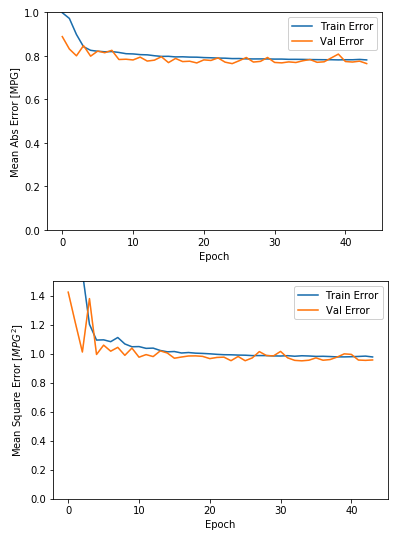
\includegraphics[width=2in]{NNComplex.png}
        \caption{Mean squared error and mean absolute error for neural network with four hidden layers.}
        \label{neuralnetcomplex}
    \end{center}
\end{figure}
The second method we tried with data generated using word2vec is \(k\)-nearest neighbours. The model used
Euclidean distance, with weights to be the inverse of distance between the test point and the neighbours.
The result is again disappointing. The model gives the best MSE to be around 0.98 when k = 500.

\subsection{Singular Value Decomposition (SVD)}

Interestingly enough, it was not necessary to process the training data in order to use the SVD algorithm.
Running Python Surprise's SVD on the entire raw training data without any hyper-parameter tuning resulted in an
initial RMSE of 0.86, which was already significantly better than all of our other models on our processed data.
It appears that the algorithm was able to find similarities between past user ratings without needing
any additional information on the movies themselves.

Since this was extremely promising, we decided to create an ensemble of equally-weighted SVD models, and we
increased the number of epochs that they were trained. Our results are shown below.
\begin{center}
    \begin{tabular}{c|c|c}
        Models & Epochs & RMSE\\
        \hline
        1 & 20 & 0.86054\\
        15 & 30 & 0.84404\\
        50 & 35 & 0.84181
    \end{tabular}
\end{center}

We decided against further increasing the ensemble size given that it appeared we were obtaining diminishing returns.

\section{Experiment Design and Evaluation}

Our attempt to generate predictions using word2vec data was not successful. One of the plausible reasons was that this
approach rates movies solely on the relationship between one user vector and one movie vector, while more successful
algorithms we have tried involved elements of collaborative filtering. Thus, our successful models all trained on
a form of \{movie, user\} feature vector pairs rather than word2vec data.

To assess each different model's accuracy, we used the root mean square error (RMSE) shown below:
\[\text{Error}=\sqrt{\frac{1}{n}\sum_{i=1}^N (y_{i,predicted}-y_{i,actual})^2}\]
This error metric is the same as the contest error metric. Most notably, it penalized larger errors significantly more than smaller errors.
Using this error metric, we found the test error of all our top models in the table below, sorted in order of increasing MSE.
\begin{center}
    \begin{tabular}{c|c}
         Model & Score\\
         \hline
         SVD & 0.84181\\
         Random Forest & 0.89190\\
         GBT & 0.91087\\
         Linear Regression & 0.92219\\
         Average & 0.92798\\
         Neural Network & 0.93552
    \end{tabular}
\end{center}
From these results, it's clear that the SVD ensemble model is by far the most accurate for movie rating predictions.

\section{Conclusion}

Our research aim was to predict the rating that a user gave to a movie when given an unseen \{user, movie\} pair.
We also had to perform better than peers in a Kaggle competition, and we did fairly well. We ranked 10th out
of 18 in the leaderboards with a score of  0.84181. We approached this problem by reading the necessary data from the provided CSV files,
visualizing this data for insight, and processing the data into \{movie, user\} feature vectors and alternatively
as word2vec feature vectors. Next, we iteratively trained and tuned a random forest mode, a gradient boosted tree
model, a linear regression model, a neural network, as well as a SVD ensemble model using this data. We found most
success with our SVD ensemble at an RMSE testing error of around 0.84. In the future, this model could be further
improved with more user ratings data as well as new user browsing data. Using this and other recommendation system
models, we will be able to improve the success of the movie industry by providing movie enthusiasts with better options.

\section{Task Distribution}

\begin{center}
    \begin{tabular}{c|c}
        Task & Person \\
        \hline
        Visualization & Jennie, Alex \\
        Data Cleaning and Processing & Michael, Yijing, Alex\\
        Random Forest & Michael \\
        GBT & Danny \\
        Word2Vec Algorithm & Yijing \\
        Neural Networks & Michael, Yijing \\
        SVD & Danny \\
        Linear Regression & Michael\\
        Average & Alex\\
        Report & Everyone \\
    \end{tabular}
\end{center}

\section{References}

\begin{enumerate}
    \item Emmanuel, O. (2018, March). Day 1: Building a
    Recommendation System Using Machine Learning (ML) and Artificial Intelligence.
    \href{https://medium.com/the-happiness-of-pursuit/day-1-building-a-recommendation-system-using-machine-
    learning-ml-and-artificial-intelligence-c8b2c5ef53a8}{Link}.

    \item Sarwar, B. M., Karypis, G., Konstan, J., \& Riedl, J. (2002, December).
    Recommender systems for large-scale e-commerce: Scalable neighborhood formation using
    clustering. In Proceedings of the fifth international conference on computer and information technology (Vol. 1, pp. 291-324).

    \item Spark, C. (2018, October). Tutorial: Practical Introduction to Recommender
    Systems. \href{https://blog.cambridgespark.com/tutorial-practical-introduction-to-recommender-systems-dbe22848392b}{Link}.
\end{enumerate}

\end{document}